\documentclass{beamer}
\usepackage[T1]{fontenc}
\usepackage[utf8]{inputenc}
\usepackage{lmodern}
\usepackage[brazil]{babel}
\usepackage[labelformat=empty]{caption}
\usepackage{graphicx}
\usepackage{color}

\definecolor{beamer@blendedblue}{rgb}{0.5, 0.6, 0.4}
\definecolor{covered}{gray}{0.65}
\definecolor{filecolor}{rgb}{0, 0.3, 0.7}
\usetheme{Warsaw}
\title[NetSim: um simulador de redes simplificado.]{NetSim: um simulador de redes simplificado.}
\author{Carlos Eduardo Leão Elmadjian \and Renan Fichberg}
\date{25 de Novembro de 2014}
\institute{Instituto de Matemática e Estatística da Universidade de São Paulo (IME-USP)}

\expandafter\def\expandafter\insertshorttitle\expandafter{%
\insertshorttitle\hfill%
\insertframenumber\,/\,\inserttotalframenumber}

\begin{document}

\begin{frame}
	\titlepage
\end{frame}

\begin{frame}
\begin{center}
	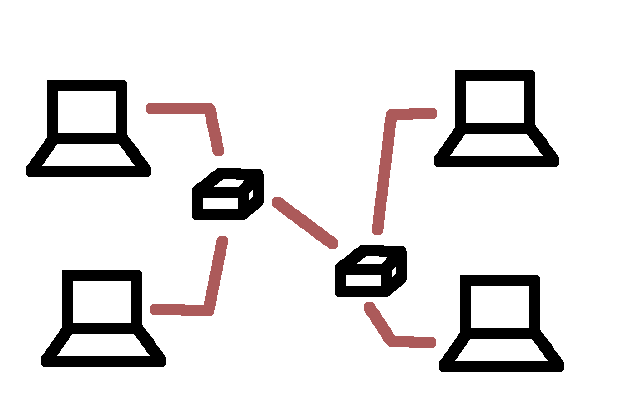
\includegraphics[scale=0.3]{simulator.png}
\end{center}
\end{frame}

\begin{frame}
	\frametitle{Conteúdo}
	\begin{itemize}
		\item O simulador: como funciona?
		\item Testes realizados com o simulador
		\item Dificuldades encontradas
	\end{itemize}
\end{frame}

\begin{frame}
	\frametitle{O simulador: como funciona?}
	\begin{itemize}
		\item Estrutura do NetSim
		\item Entradas
		\item Saídas
		\item As classes e as suas funções
	\end{itemize}
\end{frame}

\begin{frame}
	\frametitle{O simulador: como funciona?}
	\framesubtitle{Estrutura do NetSim}
	O NetSim é dividido em módulos. Isso foi pensado desta maneira pois, logo de inicio, 
	foi imaginado que haveriam muitas classes. Como o programa foi desenvolvido em Java, ao compilá-lo, 
	há um boom na quantidade de arquivos com o surgimento dos de extensão .class. 
	Com isto, para diminuir o caos no diretório que contém o código-fonte, há outros
	dois sub-diretórios:
	\begin{itemize}
		\item \textbf{/inputs} - Contém arquivos .txt com entradas para alimentar o simulador. É aqui que o usuário deve deixar suas entradas, \textbf{obrigatoriamente}.
		\item \textbf{/logs} - Contém arquivos .log com as saídas. As saídas são os pacotes capturados pelos \textit{Sniffers} definidos na entrada que alimentou o programa.
	\end{itemize}
\end{frame}

\begin{frame}
	\frametitle{O simulador: como funciona?}
	\begin{itemize}
		\item \textcolor{covered}{Estrutura do NetSim}
		\item Entradas
		\item Saídas
		\item As classes e as suas funções
	\end{itemize}
\end{frame}

\begin{frame}
	\frametitle{O simulador: como funciona?}
	\framesubtitle{Entradas}
	Há no total apenas \textbf{12} tipos de entrada esperadas pelo programa. São elas:
	\begin{itemize}
		\item Entrada para criação de computadores (\textit{hosts})
		\item Entrada para criação de roteadores (\textit{routers})
		\item Entrada para criação de enlaces do tipo duplex-link
		\item Entrada para configuração dos \textit{hosts} com relação aos endereços de IP do próprio computador, do roteador padrão e do servidor DNS
	\end{itemize}
\end{frame}

\begin{frame}
	\frametitle{O simulador: como funciona?}
	\framesubtitle{Entradas}
	\begin{itemize}
		\item Entrada para configuração dos \textit{routers} com relação às portas e aos endereços de IP
		\item Entrada para a configuração dos \textit{routers} com relação às rotas
		\item Entrada para a configuração dos \textit{routers} com relação aos seus dados de \textit{performance}
		\item Entrada para a configuração dos agentes da camada de aplicação: declaração do agente e da sua natureza 
	\end{itemize}
\end{frame}

\begin{frame}
	\frametitle{O simulador: como funciona?}
	\framesubtitle{Entradas}
	\begin{itemize}
		\item Entrada para a configuração dos agentes da camada de aplicação: associação do agente declarado a um \textit{host}
		\item Entrada para a configuração dos agentes da camada de aplicação: declaração dos \textit{sniffers}
		\item Entrada para a configuração dos agentes da camada de aplicação: locais da rede onde os \textit{sniffers} agirão.
		\item Entrada para a Configuração das comunicações entre os agentes.
	\end{itemize}
\end{frame}

\begin{frame}
	\frametitle{O simulador: como funciona?}
	\begin{itemize}
		\item \textcolor{covered}{Estrutura do NetSim}
		\item \textcolor{covered}{Entradas}
		\item Saídas
		\item As classes e as suas funções
	\end{itemize}
\end{frame}

\begin{frame}
	\frametitle{O simulador: como funciona?}
	\framesubtitle{Saídas}
	As saídas, como já mencionado anteriormente, são os resultados das capturas dos pacotes pelo \textit{sniffers}, e estas
	ficam armazenadas por default no sub-diretório de logs. Cada \textit{sniffer} tem seu próprio log, cujo o nome do arquivo tem o formato
	\textbf{nome\_do\_sniffer.log}. Este é o comportamento do programa para caso o usuário não passe uma saída da sua escolha. 
\end{frame}

\begin{frame}
	\frametitle{O simulador: como funciona?}
	\framesubtitle{Saídas}
	O formato da saída é o seguinte:
	\begin{itemize}
		\item Identificador do pacote
		\item Instante de tempo em que o pacote foi visto (a partir da execução do programa)
		\item Identificador do \textit{sniffer}
		\item Informações da camada de rede (IP):
		\begin{itemize}
			\item IP de origem
			\item IP de destino
			\item Identificação do protocolo da camada acima
			\item Tamanho cabeçalho IP + tamanho das camadas superiores
			\item TTL
		\end{itemize}
	\end{itemize}
\end{frame}

\begin{frame}
	\frametitle{O simulador: como funciona?}
	\framesubtitle{Saídas}
	\begin{itemize}
		\item Informações da camada de transporte (se for TCP):
		\begin{itemize}
			\item Porta origem
			\item Porta destino
			\item Tamanho cabeçalho TCP + tamanho da camada superior
			\item Número de Seqüência
			\item Número de Reconhecimento
			\item Bit ACK
			\item Bit FIN
			\item Bit SYN
		\end{itemize}
		\item Informações da camada de transporte (se for UDP):
		\begin{itemize}
			\item Porta origem
			\item Porta destino
			\item Tamanho cabeçalho UDP + tamanho da camada superior
		\end{itemize}
	\end{itemize}
\end{frame}

\begin{frame}
	\frametitle{O simulador: como funciona?}
	\framesubtitle{Saídas}
	\begin{itemize}
		\item Informações da camada de aplicação (DNS/FTP/HTTP):
		\begin{itemize}
			\item Pergunta ou resposta contida no pacote.
		\end{itemize}
	\end{itemize}
	Ainda, além das informações estarem presentes no log, a cada captura os resultados daquele \textit{sniffer}
	são imprimidos no \textit{prompt} em tempo de execução.
\end{frame}

\begin{frame}
	\frametitle{O simulador: como funciona?}
	\begin{itemize}
		\item \textcolor{covered}{Estrutura do NetSim}
		\item \textcolor{covered}{Entradas}
		\item \textcolor{covered}{Saídas}
		\item As classes e as seus papeis
	\end{itemize}
\end{frame}

\begin{frame}
	\frametitle{O simulador: como funciona?}
	\framesubtitle{As classes e as suas funções}
	\begin{itemize}
		\item Agent: classe abstrata que representa um agente da rede
		\item ApplicationLayer: classe que representa uma camada de aplicação
		\item Clock: classe responsável pelo tempo de execução
		\item DNSServer: classe que representa um servidor DNS
		\item DuplexLink: classe que representa um enlace do tipo \textit{duplex-link}
	\end{itemize}
\end{frame}

\begin{frame}
	\frametitle{O simulador: como funciona?}
	\framesubtitle{As classes e as suas funções}
	\begin{itemize}
		\item FTPClient: classe que representa um cliente FTP
		\item FTPServer: classe que representa um servidor FTP
		\item Host: classe que representa um \textit{host} da rede
		\item HTTPClient: classe que representa um cliente HTTP
		\item HTTPServer: classe que representa um servidor HTTP
	\end{itemize}
\end{frame}

\begin{frame}
	\frametitle{O simulador: como funciona?}
	\framesubtitle{As classes e as suas funções}
	\begin{itemize}
		\item InputReader: classe responsavel por manipular os arquivos de entrada do simulador
		\item NetSim: classe que representa o simulador de redes
		\item Node: classe que representa um nó. Um nó pode ser tanto um \textit{host} quanto um \textit{router}
		\item Packet: classe que representa um pacote
		\item Router: classe que representa um \textit{router} da rede 
	\end{itemize}
\end{frame}

\begin{frame}
	\frametitle{O simulador: como funciona?}
	\framesubtitle{As classes e as suas funções}
	\begin{itemize}
		\item RouterBuffer: classe que representa um buffer do \textit{router}. Funciona em FIFO
		\item SimulatorLogger: classe responsável por escrever os arquivos de saída
		\item Sniffer: classe que representa um \textit{sniffer}
		\item TCP: classe que armazena os dados do TCP na camada de transporte
		\item TransportLayer: classe abstrata que representa uma camada de transporte
		\item UDP: classe que armazena os dados do UDP na camada de transporte
	\end{itemize}
\end{frame}

\begin{frame}
	\frametitle{O simulador: como funciona?}
	\begin{itemize}
		\item \textcolor{covered}{Estrutura do NetSim}
		\item \textcolor{covered}{Entradas}
		\item \textcolor{covered}{Saídas}
		\item \textcolor{covered}{As classes e as seus papeis}
	\end{itemize}
\end{frame}

\begin{frame}
	\frametitle{Conteúdo}
	\begin{itemize}
		\item \textcolor{covered}{O simulador: como funciona?}
		\item Testes realizados com o simulador
		\item Dificuldades encontradas
	\end{itemize}
\end{frame}

\begin{frame}
	\frametitle{Testes realizados com o simulador}
	Aqui serão apresentados gráficos dos testes. O valor da barra representado nas imagens é a \textbf{média}.
	Mais informações podem ser encontradas no arquivo \textbf{testes.txt}. Valores medidos para um intervalo de confiança de 95\%.
\end{frame}

\begin{frame}
	\frametitle{Testes realizados com o simulador}
	\framesubtitle{Cenário simples - Tempo}
	\begin{center}
	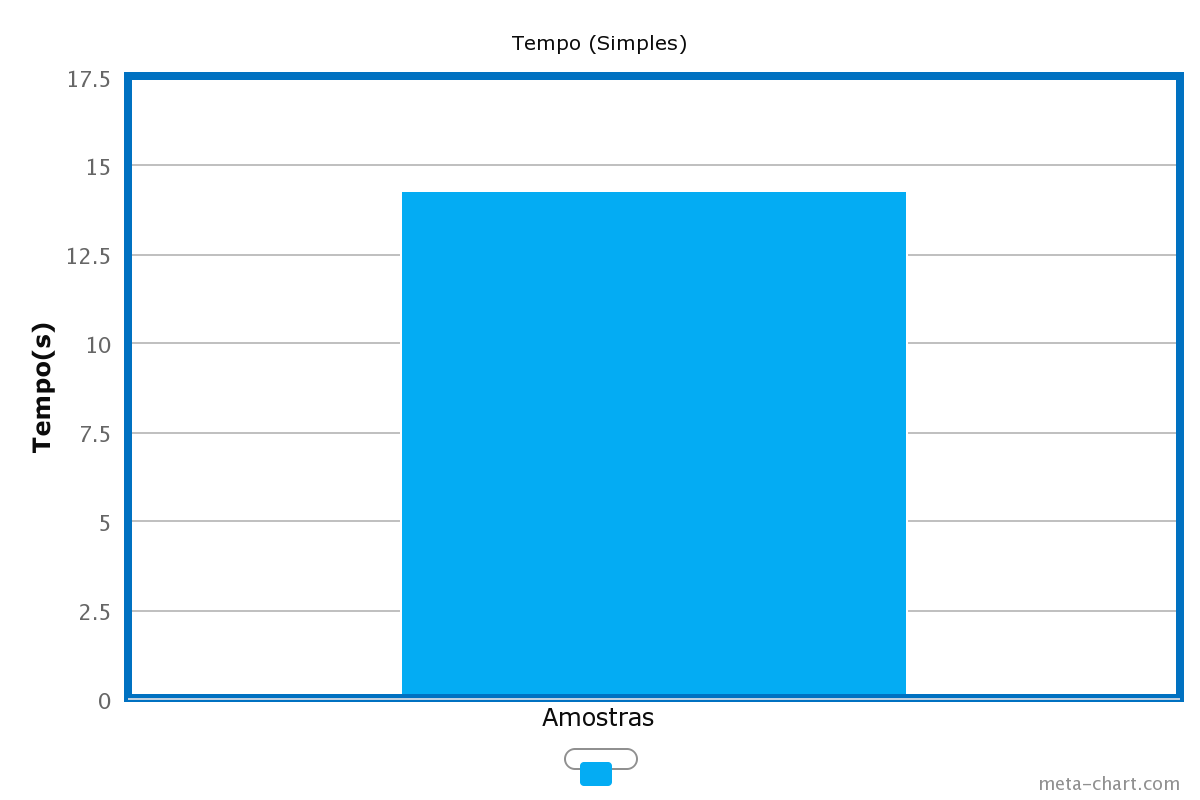
\includegraphics[scale=0.18]{chart.png}
	\end{center}
	\begin{center}
	Média = 14.3107
	\end{center}
	\begin{center}
	IC = [14.294149138 ; 14.327250862]
	\end{center}
\end{frame}

\begin{frame}
	\frametitle{Testes realizados com o simulador}
	\framesubtitle{Cenário simples - CPU}
	\begin{center}
	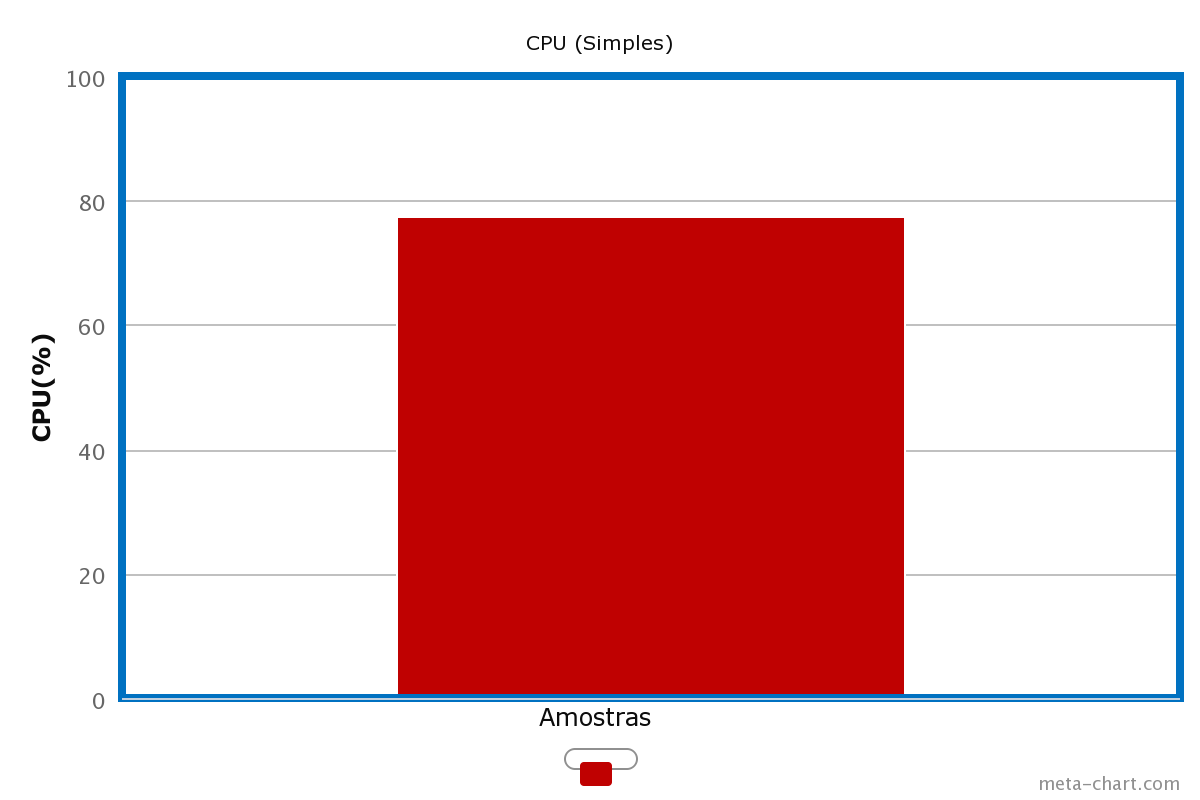
\includegraphics[scale=0.18]{chart(1).png}
	\end{center}
	\begin{center}
	Média = 77.3667
	\end{center}
	\begin{center}
	IC = [77.18370188 ; 77.54969812]
	\end{center}
\end{frame}

\begin{frame}
	\frametitle{Testes realizados com o simulador}
	\framesubtitle{Cenário intermediário - Tempo}
	\begin{center}
	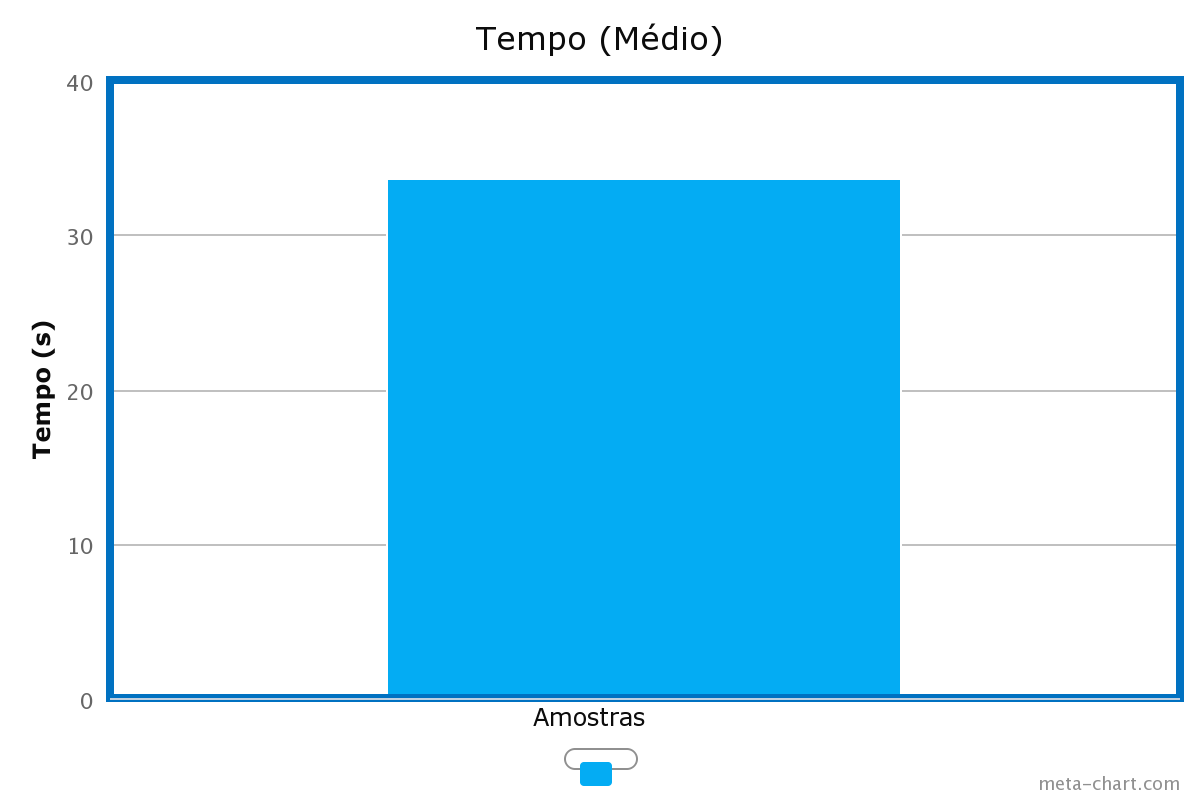
\includegraphics[scale=0.18]{chart(2).png}
	\end{center}
	\begin{center}
	Média = 33.615
	\end{center}
	\begin{center}
	IC = [33.570252673 ; 33.659747327]
	\end{center}
\end{frame}

\begin{frame}
	\frametitle{Testes realizados com o simulador}
	\framesubtitle{Cenário intermediário - CPU}
	\begin{center}
	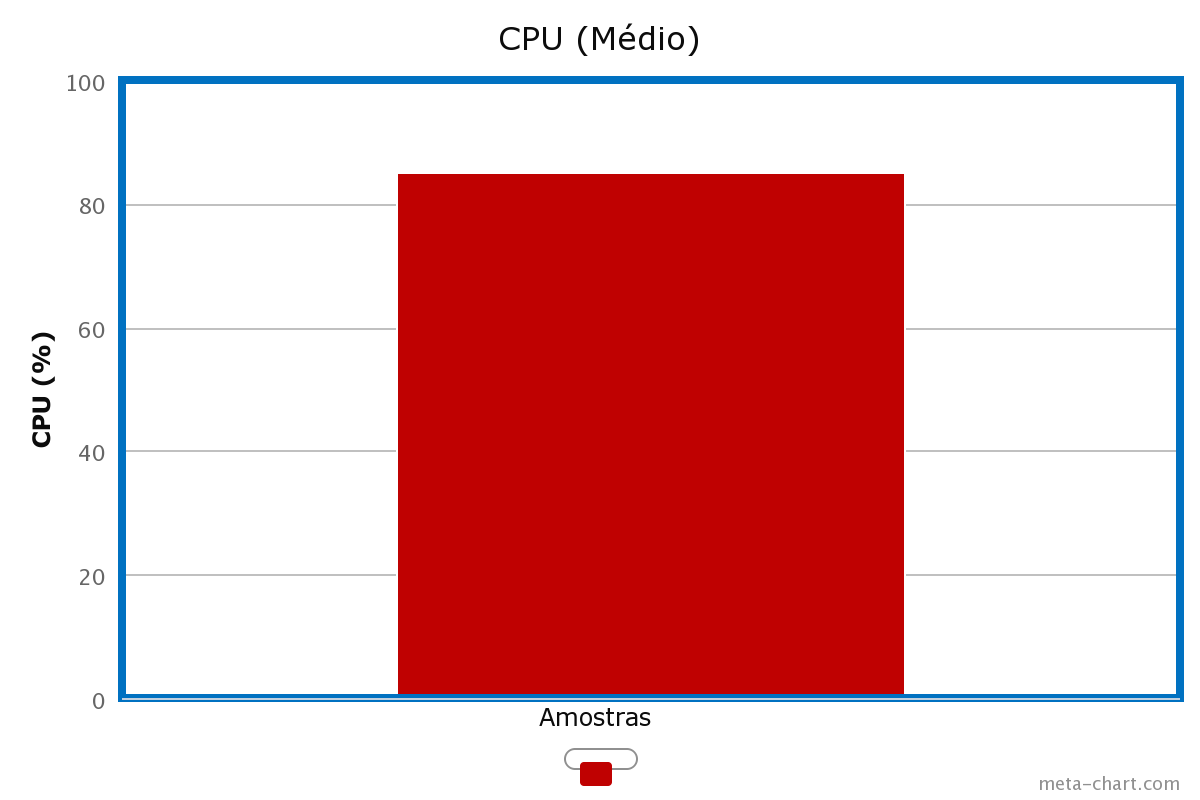
\includegraphics[scale=0.18]{chart(3).png}
	\end{center}
	\begin{center}
	Média = 85
	\end{center}
	\begin{center}
	IC = [85 ; 85]
	\end{center}
\end{frame}

\begin{frame}
	\frametitle{Testes realizados com o simulador}
	\framesubtitle{Cenário complexo - Tempo}
	\begin{center}
	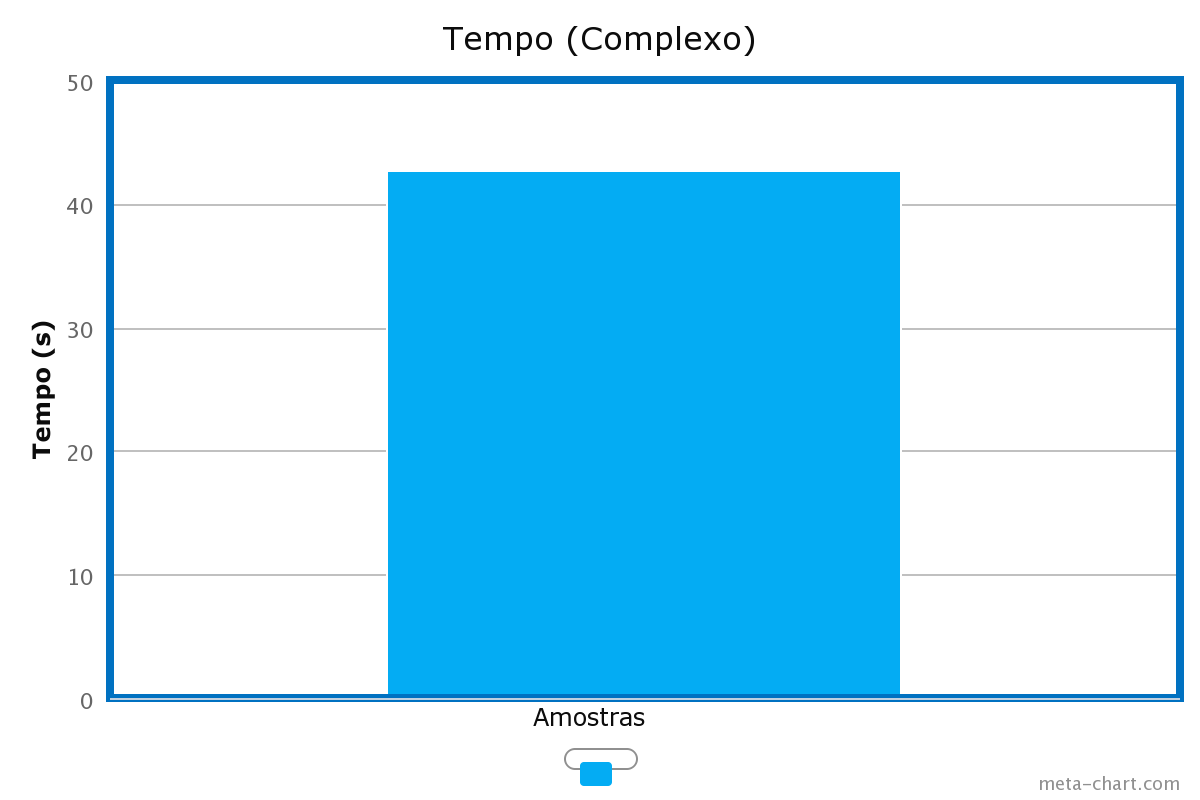
\includegraphics[scale=0.18]{chart(4).png}
	\end{center}
	\begin{center}
	Média = 42.7793
	\end{center}
	\begin{center}
	IC = [42.693827598 ; 42.864772402]
	\end{center}
\end{frame}

\begin{frame}
	\frametitle{Testes realizados com o simulador}
	\framesubtitle{Cenário complexo - CPU}
	\begin{center}
	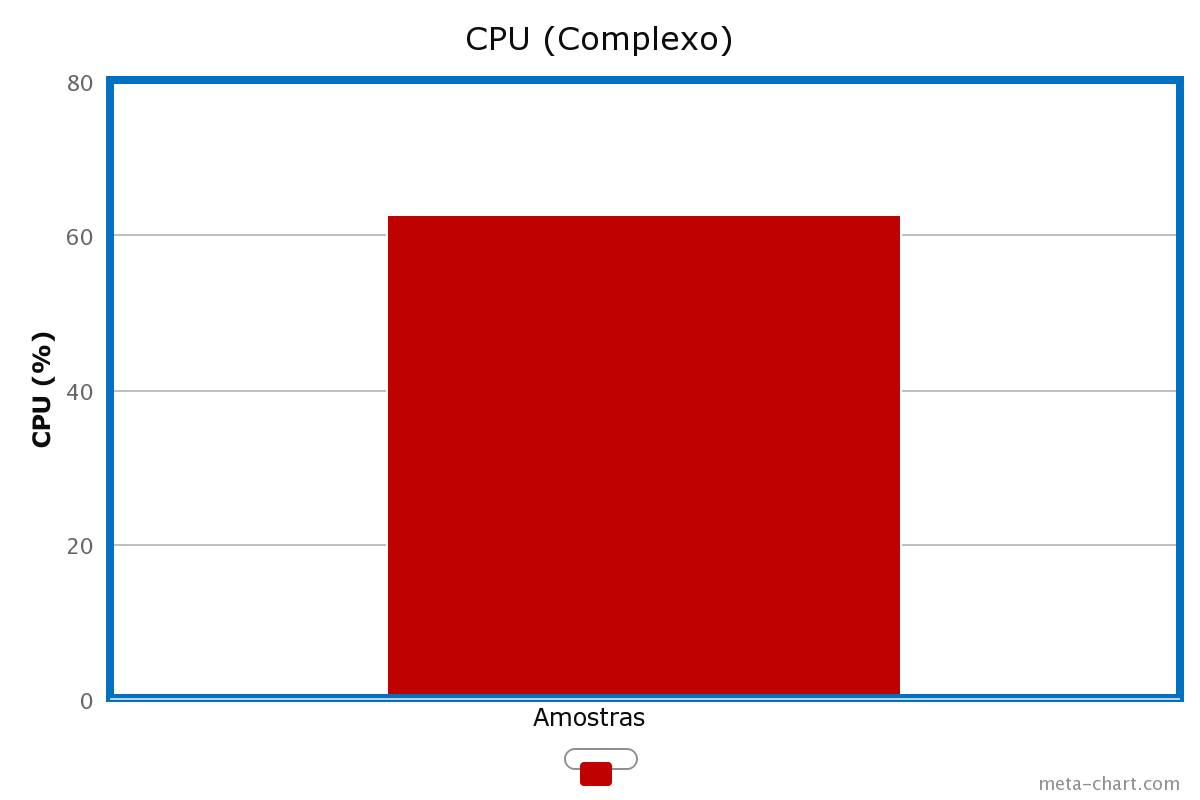
\includegraphics[scale=0.18]{chart(5).png}
	\end{center}
	\begin{center}
	Média = 62.5667
	\end{center}
	\begin{center}
	IC = [62.378521825 ; 62.754878175]
	\end{center}
\end{frame}

\begin{frame}
	\frametitle{Testes realizados com o simulador}
	\framesubtitle{Os três cenários de tempo}
	\begin{center}
	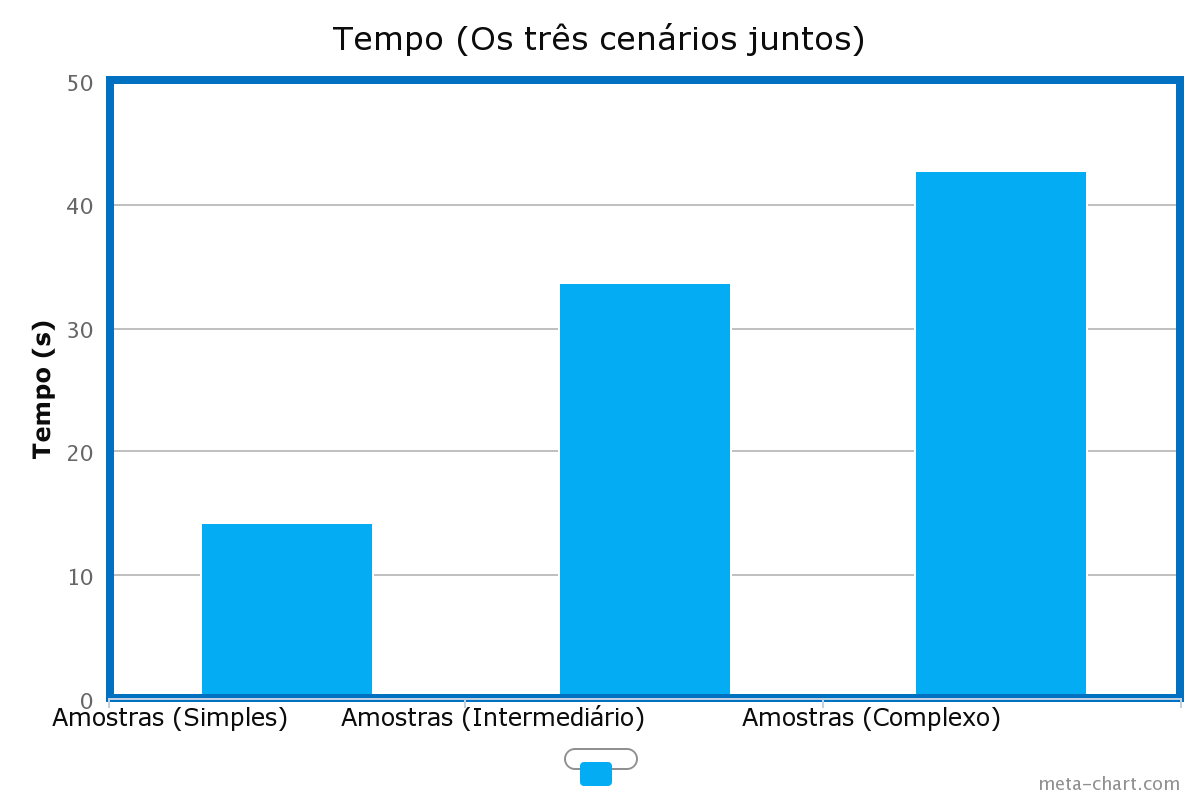
\includegraphics[scale=0.18]{chart(6).png}
	\end{center}
\end{frame}

\begin{frame}
	\frametitle{Testes realizados com o simulador}
	\framesubtitle{Os três cenários de CPU}
	\begin{center}
	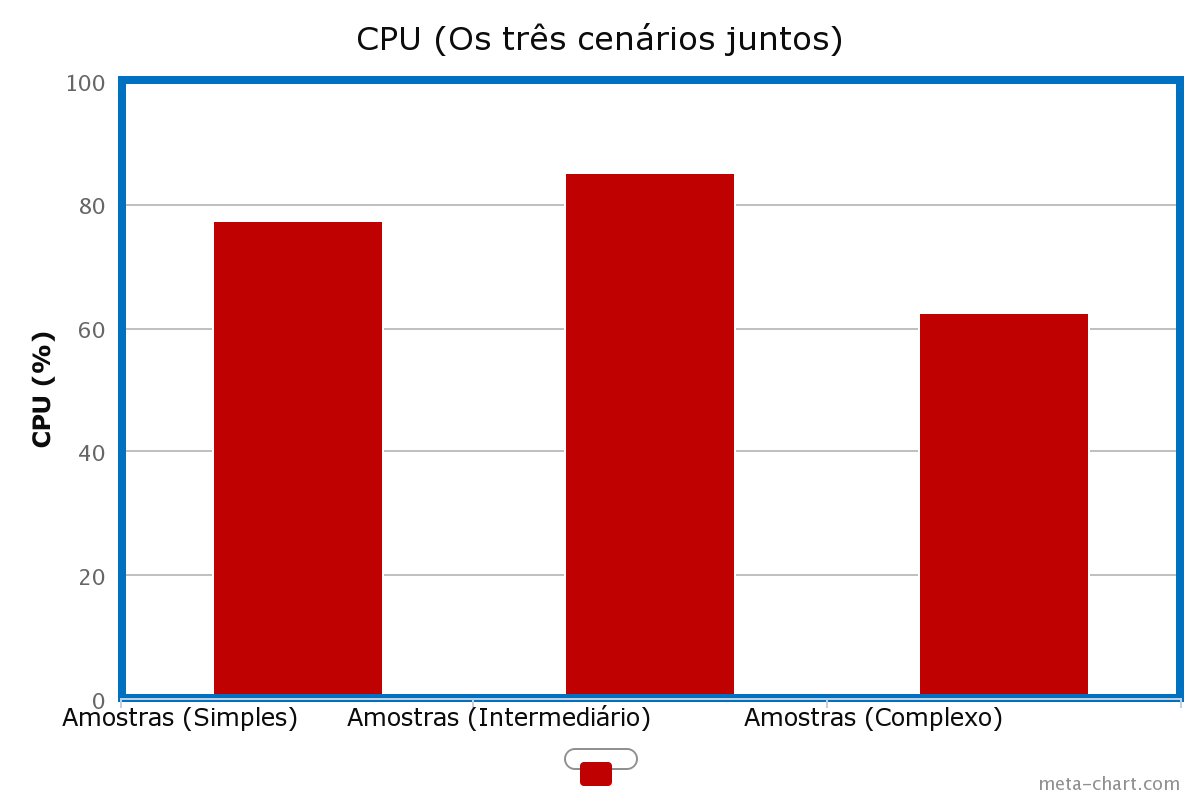
\includegraphics[scale=0.18]{chart(7).png}
	\end{center}
\end{frame}

\begin{frame}
	\frametitle{Testes realizados com o simulador}
	\framesubtitle{Análise}
	\begin{itemize}
		\item 
	\end{itemize}
\end{frame}

\begin{frame}
	\frametitle{Testes realizados com o simulador}
	\framesubtitle{Informações das máquinas do experimento}
	\begin{itemize}
		\item Máquina real:
			\begin{itemize}
				\item Intel i5 2500K 3.3GHz, 8GB de RAM
				\item Placa de rede Realtek RTL8111/8168/8411 – 1Gbit/s
				\item HD Seagate 7200RPM 1TB
				\item Sistema Operacional: Arch Linux x86\_64 (kernel 3.16.3-1)
			\end{itemize}
	\end{itemize}
\end{frame}

\begin{frame}
	\frametitle{Testes realizados com o simulador}
	\framesubtitle{Informações das máquinas do experimento}
	\begin{itemize}
		\item Máquina virtual:
			\begin{itemize}
				\item 1 processador da máquina hospedeira, 2GB de RAM
				\item Placa de rede em modo bridge
				\item Sistema Operacional: Elementary OS x86\_32 (kernel 3.2.0-7)
			\end{itemize}
	\end{itemize}
\end{frame}

\begin{frame}
	\frametitle{Conteúdo}
	\begin{itemize}
		\item \textcolor{covered}{O simulador: como funciona?}
		\item \textcolor{covered}{Testes realizados com o simulador}
		\item Dificuldades encontradas
	\end{itemize}
\end{frame}

\begin{frame}
	\frametitle{Dificuldades encontradas e pontos positivos}
	Dificuldades:
	\begin{itemize}
		\item Planejamento: encontrar a estrutura ideal que comporte os seis protocolos requisitados
		\item Concorrência: encontrar a forma ideal para lidar com todos os pacotes circulando pela rede simultaneamente
		\item Integração entre todas as classes do programa
	\end{itemize}
\end{frame}

\begin{frame}
	\frametitle{Dificuldades encontradas e pontos positivos}
	Pontos positivos:
	\begin{itemize}
		\item Aprendizado: mais conhecimento sobre o funcionamento das camadas e como elas interagem
		\item Menos problemas para planejar a estrutura do programa graças a bagagem do EP2
	\end{itemize}
\end{frame}

\begin{frame}
	\frametitle{Conteúdo}
	\begin{itemize}
		\item \textcolor{covered}{O simulador: como funciona?}
		\item \textcolor{covered}{Testes realizados com o simulador}
		\item \textcolor{covered}{Dificuldades encontradas e pontos positivos}
	\end{itemize}
\end{frame}

\begin{frame}
	\frametitle{Conteúdo}
	\begin{center}
	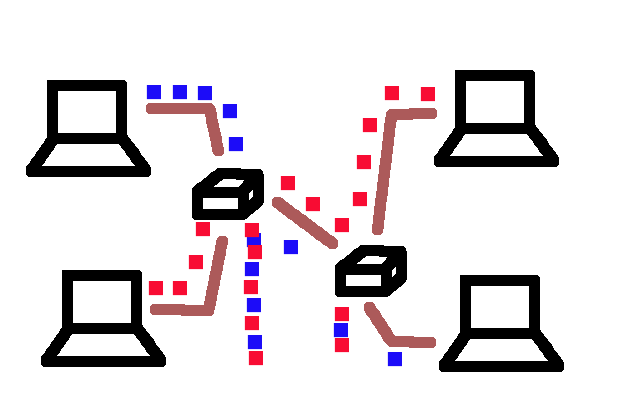
\includegraphics[scale=0.3]{simulator2.png}
	\end{center}
	\begin{center}
	Obrigado! :)
	\end{center}

\end{frame}

\end{document}